% main.tex
% Main document for Lab04 exercises
% Comprehensive demonstration of LaTeX graphics and floats

\documentclass[12pt]{article}
\usepackage[T1]{fontenc}
\usepackage[utf8]{inputenc}
\usepackage{graphicx}
\usepackage{lipsum}
\usepackage{float}
\usepackage{geometry}
\usepackage{hyperref}
\usepackage{caption}
\usepackage{subcaption}
\usepackage{booktabs}
\usepackage{array}

% Set page margins
\geometry{a4paper, margin=1in}

% Set graphics path
\graphicspath{{figures/}}

% Document information
\title{Lab04: Graphics and Floats in \LaTeX}
\author{Nadia Ezzakate}
\date{\today}

\begin{document}

\maketitle
\tableofcontents
\newpage

\section{Introduction}
This document demonstrates various aspects of including graphics and managing floats in \LaTeX, as requested in the lab04 exercises. Each section addresses a specific exercise requirement.

\section{Exercise 1: Including Custom Images}
\label{sec:exercise1}

This section demonstrates including custom-created images in different formats.

\subsection{Including a PNG Image}
\begin{figure}[h]
    \centering
    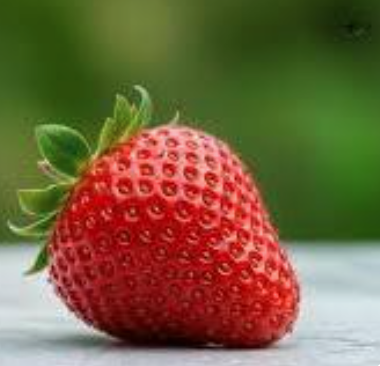
\includegraphics[width=0.6\textwidth]{image.png}
    \caption{Custom PNG image created for this lab}
    \label{fig:custom-png}
\end{figure}

\subsection{Including a PDF Image}
\begin{figure}[h]
    \centering
    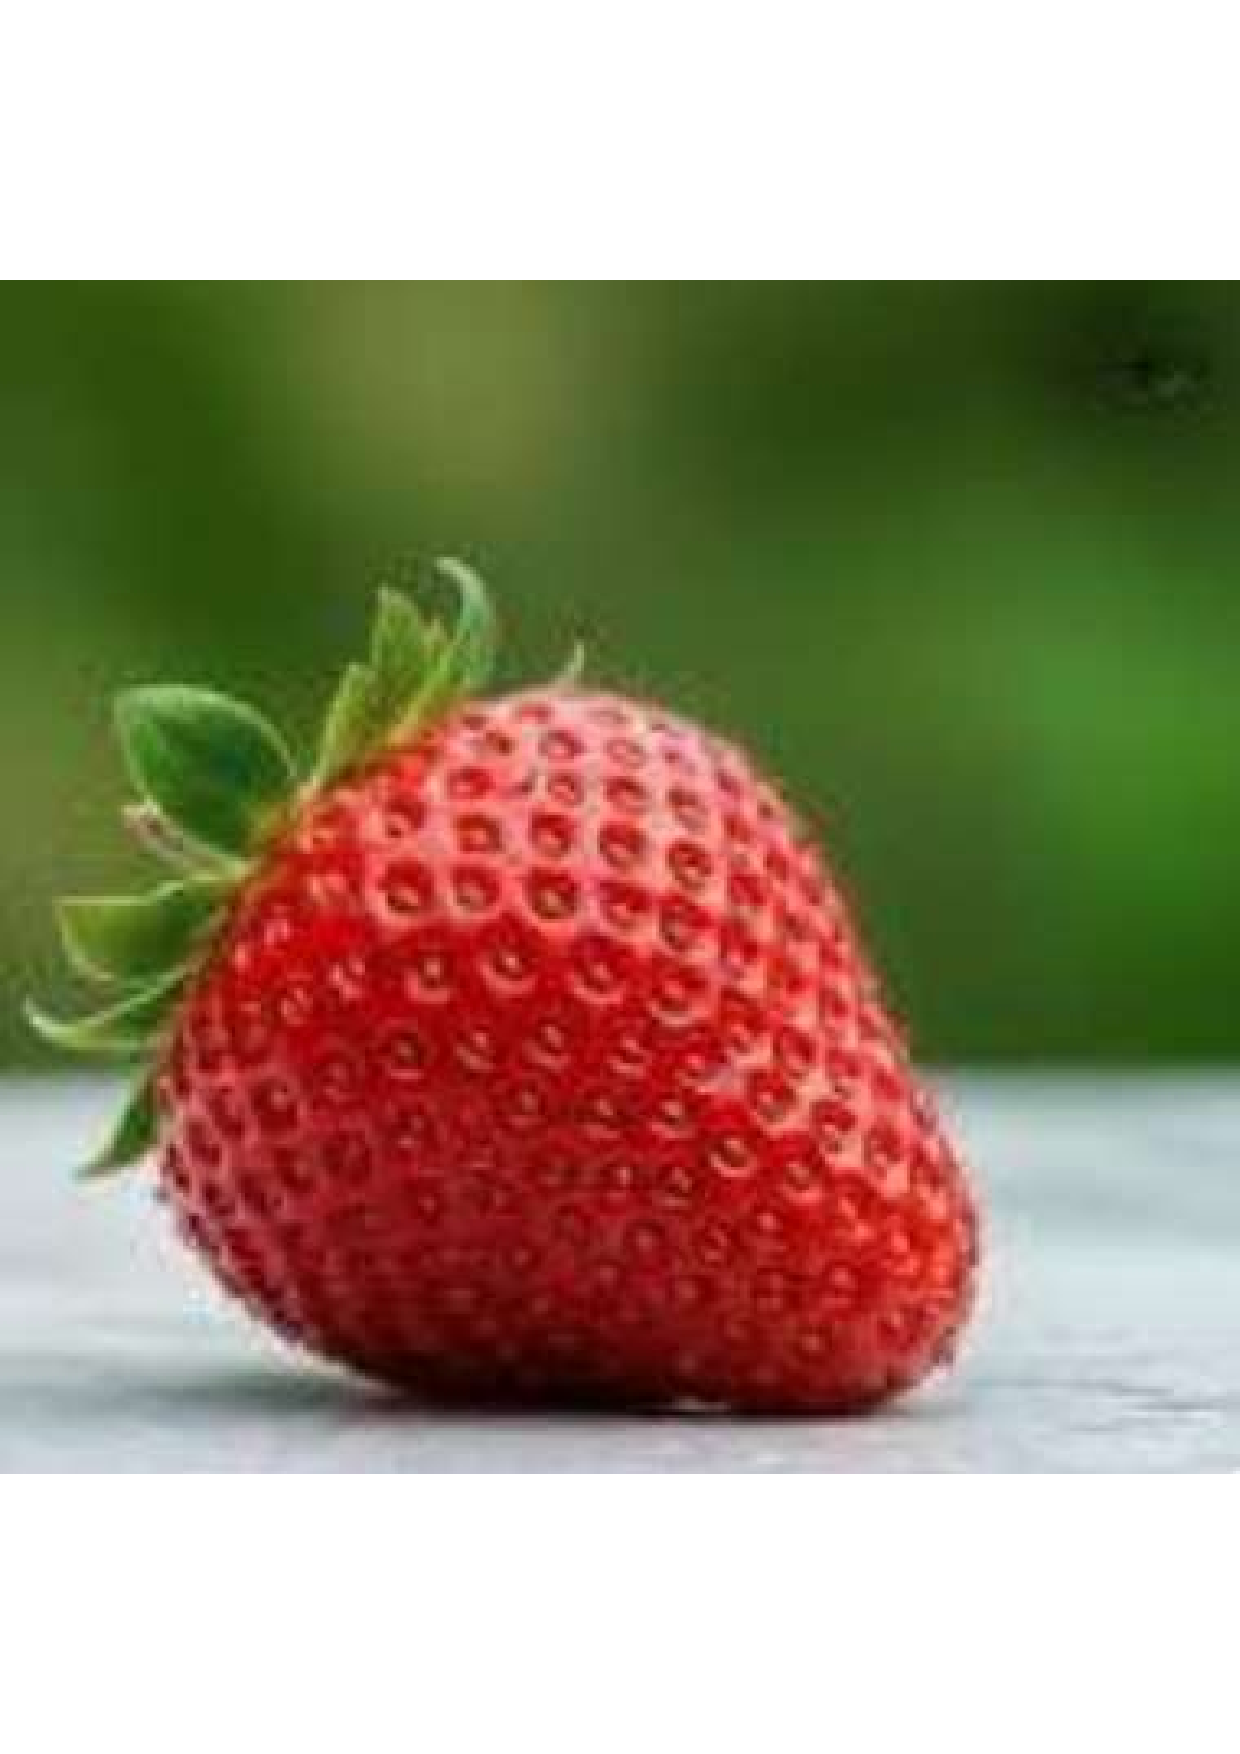
\includegraphics[width=0.6\textwidth]{image.pdf}
    \caption{Custom PDF image created for this lab}
    \label{fig:custom-pdf}
\end{figure}

\subsection{Multiple Images Side by Side}
\begin{figure}[h]
    \centering
    \begin{subfigure}{0.45\textwidth}
        \centering
        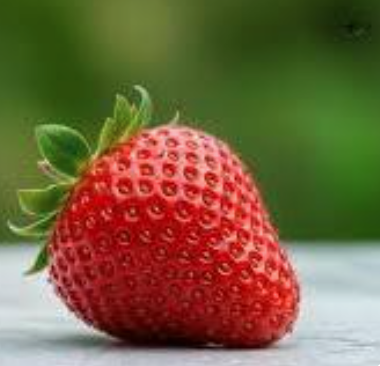
\includegraphics[width=\textwidth]{image.png}
        \caption{PNG version}
        \label{fig:sub-png}
    \end{subfigure}
    \hfill
    \begin{subfigure}{0.45\textwidth}
        \centering
        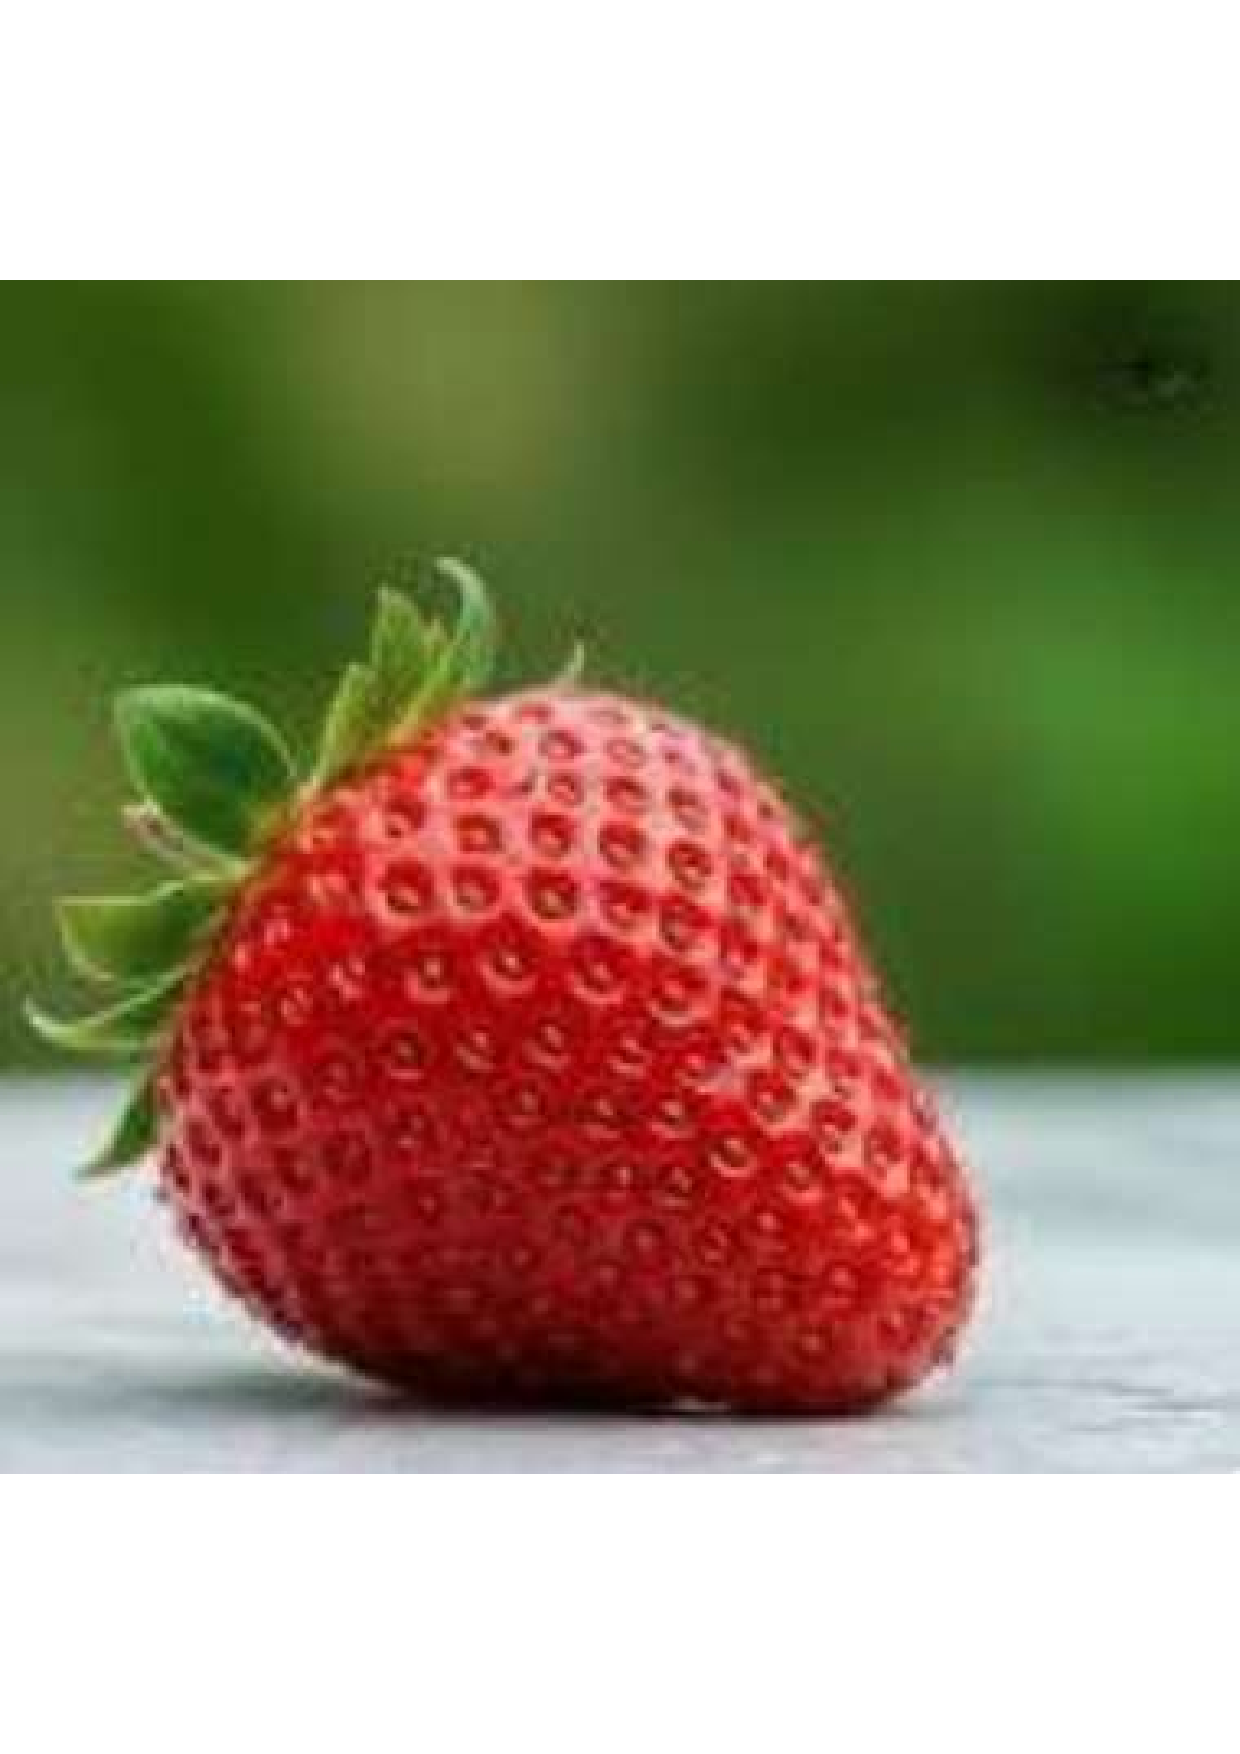
\includegraphics[width=\textwidth]{image.pdf}
        \caption{PDF version}
        \label{fig:sub-pdf}
    \end{subfigure}
    \caption{Comparison of PNG and PDF image formats}
    \label{fig:side-by-side}
\end{figure}

\newpage
\section{Exercise 2: Exploring Image Options}
\label{sec:exercise2}

This section demonstrates various options for manipulating images: height, width, angle, and scale.

\subsection{Height and Width Options}
\begin{figure}[h]
    \centering
    \begin{subfigure}{0.3\textwidth}
        \centering
        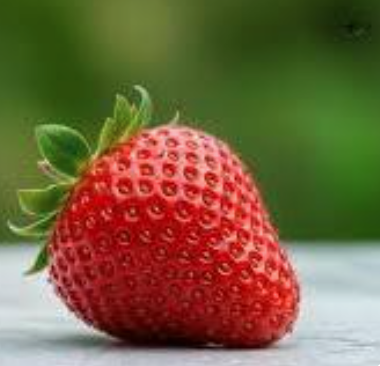
\includegraphics[height=3cm]{image.png}
        \caption{height=3cm}
    \end{subfigure}
    \hfill
    \begin{subfigure}{0.3\textwidth}
        \centering
        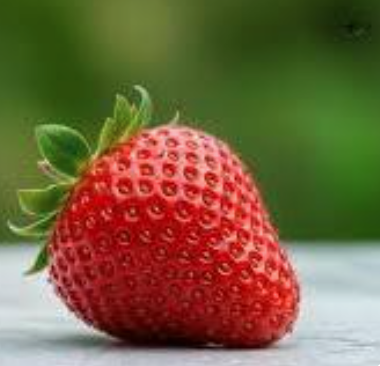
\includegraphics[width=3cm]{image.png}
        \caption{width=3cm}
    \end{subfigure}
    \hfill
    \begin{subfigure}{0.3\textwidth}
        \centering
        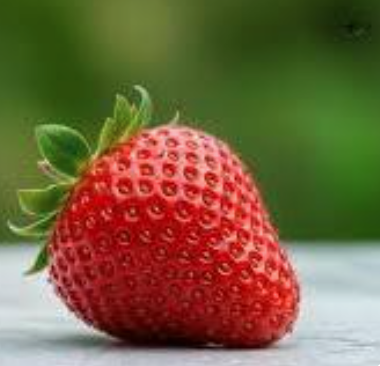
\includegraphics[height=3cm,width=3cm]{image.png}
        \caption{both (distorted)}
    \end{subfigure}
    \caption{Different dimension specifications}
\end{figure}

\subsection{Rotation Options}
\begin{figure}[h]
    \centering
    \begin{subfigure}{0.3\textwidth}
        \centering
        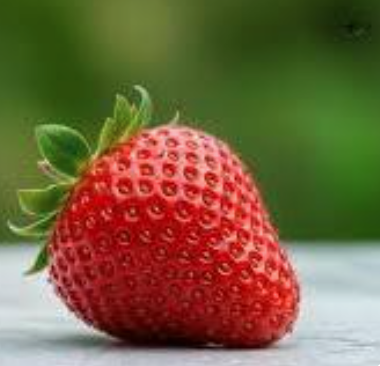
\includegraphics[width=3cm,angle=45]{image.png}
        \caption{angle=45°}
    \end{subfigure}
    \hfill
    \begin{subfigure}{0.3\textwidth}
        \centering
        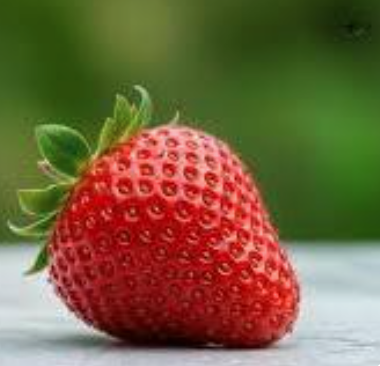
\includegraphics[width=3cm,angle=90]{image.png}
        \caption{angle=90°}
    \end{subfigure}
    \hfill
    \begin{subfigure}{0.3\textwidth}
        \centering
        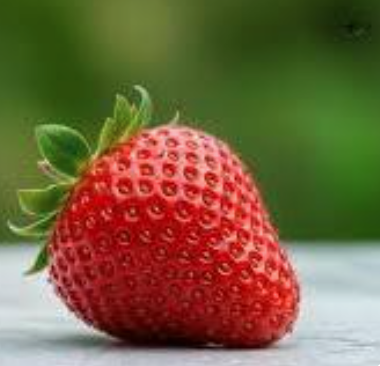
\includegraphics[width=3cm,angle=180]{image.png}
        \caption{angle=180°}
    \end{subfigure}
    \caption{Rotation effects}
\end{figure}

\subsection{Scale Options}
\begin{figure}[h]
    \centering
    \begin{subfigure}{0.3\textwidth}
        \centering
        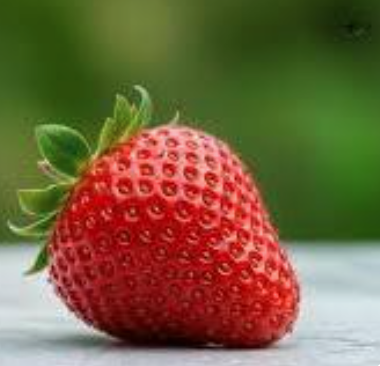
\includegraphics[scale=0.5]{image.png}
        \caption{scale=0.5}
    \end{subfigure}
    \hfill
    \begin{subfigure}{0.3\textwidth}
        \centering
        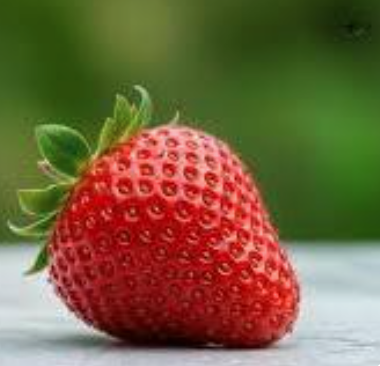
\includegraphics[scale=1.0]{image.png}
        \caption{scale=1.0}
    \end{subfigure}
    \hfill
    \begin{subfigure}{0.3\textwidth}
        \centering
        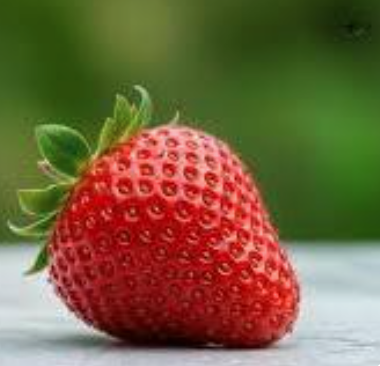
\includegraphics[scale=1.5]{image.png}
        \caption{scale=1.5}
    \end{subfigure}
    \caption{Scaling effects}
\end{figure}

\newpage
\section{Exercise 3: Relative Sizing with \textbackslash textwidth and \textbackslash linewidth}
\label{sec:exercise3}

This section demonstrates the difference between \texttt{\textbackslash textwidth} and \texttt{\textbackslash linewidth} in both single and two-column layouts.

\subsection{Single Column Mode}
\paragraph{Current settings:} 
\begin{itemize}
    \item \texttt{\textbackslash textwidth} = \the\textwidth
    \item \texttt{\textbackslash linewidth} = \the\linewidth
\end{itemize}

\begin{figure}[h]
    \centering
    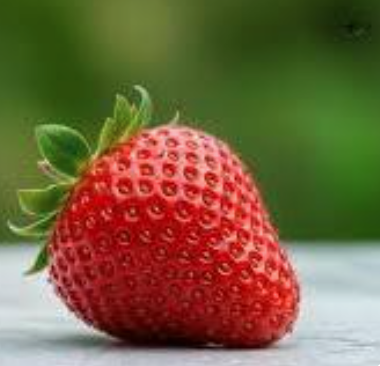
\includegraphics[width=0.5\textwidth]{image.png}
    \caption{width=0.5\textbackslash textwidth}
\end{figure}

\begin{figure}[h]
    \centering
    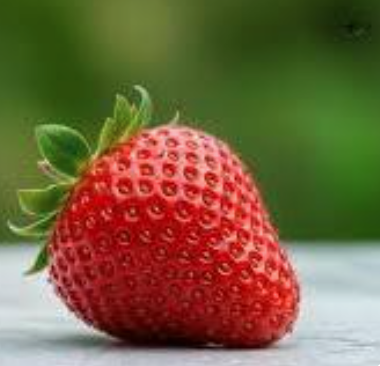
\includegraphics[width=0.5\linewidth]{image.png}
    \caption{width=0.5\textbackslash linewidth}
\end{figure}

\begin{figure}[h]
    \centering
    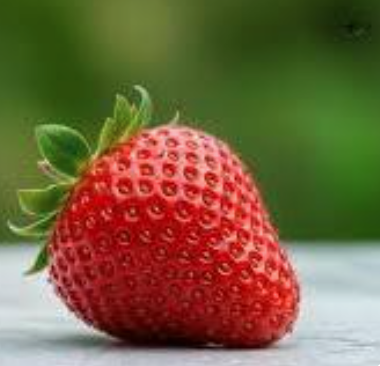
\includegraphics[width=\textwidth]{image.png}
    \caption{width=\textbackslash textwidth}
\end{figure}

\subsection{Testing with \texttt{twocolumn} Option}
To test the two-column behavior, we need to create a separate document. See the file \texttt{twocolumn\_test.tex} included in this lab folder.

\newpage
\section{Exercise 4: Float Placement with lipsum}
\label{sec:exercise4}

This section demonstrates different float placement specifiers using \texttt{lipsum} for filler text.

\subsection{Using [h] (here) specifier}
\lipsum[1-2]
\begin{figure}[h]
    \centering
    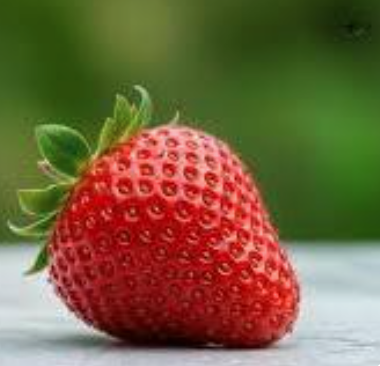
\includegraphics[width=0.6\textwidth]{image.png}
    \caption{This figure uses the [h] placement specifier}
    \label{fig:h-spec}
\end{figure}
\lipsum[3]

\subsection{Using [t] (top) specifier}
\lipsum[4]
\begin{figure}[t]
    \centering
    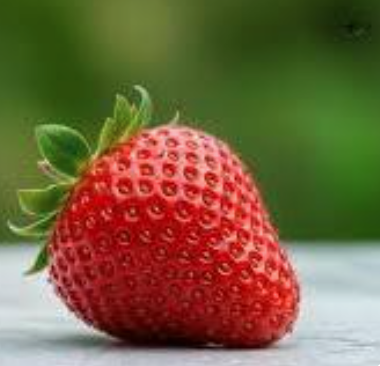
\includegraphics[width=0.6\textwidth]{image.png}
    \caption{This figure uses the [t] placement specifier}
    \label{fig:t-spec}
\end{figure}
\lipsum[5-6]

\subsection{Using [b] (bottom) specifier}
\lipsum[7]
\begin{figure}[b]
    \centering
    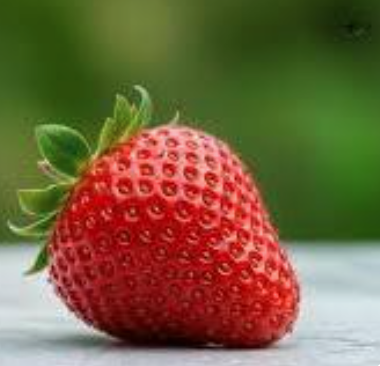
\includegraphics[width=0.6\textwidth]{image.png}
    \caption{This figure uses the [b] placement specifier}
    \label{fig:b-spec}
\end{figure}
\lipsum[8]

\subsection{Using [p] (page of floats) specifier}
\lipsum[9]
\begin{figure}[p]
    \centering
    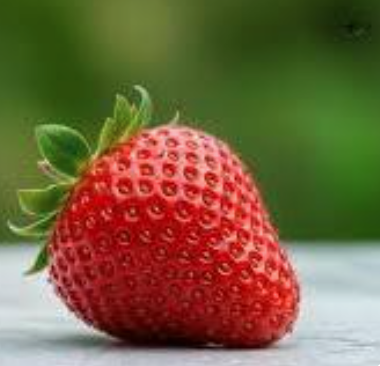
\includegraphics[width=0.6\textwidth]{image.png}
    \caption{This figure uses the [p] placement specifier}
    \label{fig:p-spec}
\end{figure}
\lipsum[10]

\subsection{Using [htbp] (all options) specifier}
\lipsum[11]
\begin{figure}[htbp]
    \centering
    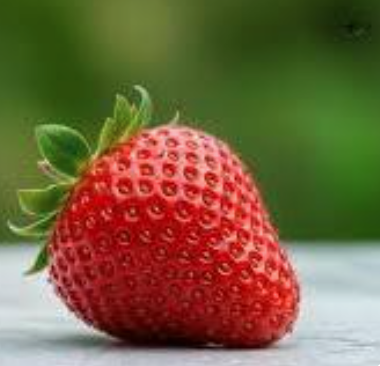
\includegraphics[width=0.6\textwidth]{image.png}
    \caption{This figure uses the [htbp] placement specifier}
    \label{fig:htbp-spec}
\end{figure}
\lipsum[12-13]

\subsection{Using [H] (absolute here) from float package}
\lipsum[14]
\begin{figure}[H]
    \centering
    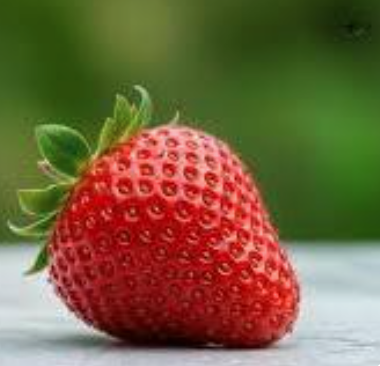
\includegraphics[width=0.6\textwidth]{image.png}
    \caption{This figure uses the [H] placement specifier from the float package}
    \label{fig:H-spec}
\end{figure}
\lipsum[15]

\newpage
\section{Exercise 5: Numbered Parts and Label Behavior}
\label{sec:exercise5}

This section demonstrates how \texttt{\textbackslash label} works with different numbered elements.

\subsection{Sections and Subsections}
\label{subsec:test-section}
This is section \ref{subsec:test-section}. Notice that the label was placed right after the subsection command.

\subsection{Enumerated Lists}
\begin{enumerate}
    \item First item \label{item:first}
    \item Second item \label{item:second}
    \item Third item \label{item:third}
\end{enumerate}

References to enumerated items: Item \ref{item:first}, Item \ref{item:second}, Item \ref{item:third}.

\subsection{Equations}
\begin{equation}
    E = mc^2 \label{eq:einstein}
\end{equation}
Equation \ref{eq:einstein} is Einstein's famous equation.

\begin{equation}
    F = ma \label{eq:newton}
\end{equation}
Equation \ref{eq:newton} is Newton's second law.


\newpage
\section{Exercise 6: Label Placement Before Caption}
\label{sec:exercise6}

This section demonstrates what happens when you place \texttt{\textbackslash label} before \texttt{\textbackslash caption}.

\subsection{Correct Label Placement (after caption)}
\begin{figure}[h]
    \centering
    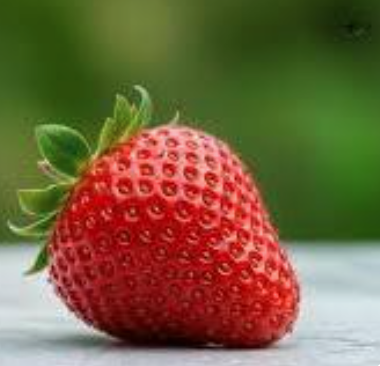
\includegraphics[width=0.6\textwidth]{image.png}
    \caption{This figure has correct label placement}
    \label{fig:correct-label}
\end{figure}
Reference to Figure \ref{fig:correct-label} works correctly.

\subsection{Incorrect Label Placement (before caption)}
\begin{figure}[h]
    \centering
    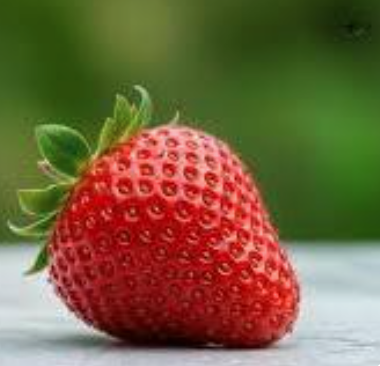
\includegraphics[width=0.6\textwidth]{image.png}
    \label{fig:incorrect-label}
    \caption{This figure has incorrect label placement}
\end{figure}
Reference to Figure \ref{fig:incorrect-label} might not work correctly (it might reference the section instead of the figure).

\subsection{Explanation}
When \texttt{\textbackslash label} comes before \texttt{\textbackslash caption}, \LaTeX\ associates the label with the previous numbered entity (in this case, the section), not with the figure. The label should always come after (or inside) the caption to refer to the figure number.

\newpage
\section{Exercise 7: Label After \textbackslash end\{equation\}}
\label{sec:exercise7}

This section demonstrates what happens when you place \texttt{\textbackslash label} after \texttt{\textbackslash end\{equation\}}.

\subsection{Correct Label Placement (inside equation)}
\begin{equation}
    \alpha^2 + \beta^2 = \gamma^2 \label{eq:correct}
\end{equation}
Reference to Equation \ref{eq:correct} works correctly.

\subsection{Incorrect Label Placement (after \textbackslash end\{equation\})}
\begin{equation}
    a^2 + b^2 = c^2
\end{equation}
\label{eq:incorrect}
Reference to Equation \ref{eq:incorrect} might not work correctly (it might reference something else).

\subsection{Explanation}
When \texttt{\textbackslash label} is placed after \texttt{\textbackslash end\{equation\}}, \LaTeX\ associates it with the previous numbered entity (like a section) rather than the equation. The label must be inside the equation environment to refer to the equation number.

\end{document}

